\documentclass[12pt, a4paper]{book}

\usepackage[utf8]{inputenc} 
\usepackage[T1]{fontenc}
\usepackage{mathpazo} 
\usepackage{algorithm}
\usepackage{algpseudocode}
\usepackage{tabularx}
\usepackage{flafter}
\usepackage{longtable}
\usepackage{float}
\usepackage{multirow}
\usepackage{multicol}
\usepackage{pgfplots}  
\usetikzlibrary{patterns}
\usepackage{emptypage}
\usepackage{hyperref}
\usepackage{tikz}
\usepackage{subfig}
\usepackage{subcaption}
\usepackage{listings}
\usepackage[square,numbers]{natbib}
\bibliographystyle{abbrvnat}

\begin{document}

    \sloppy

    \frontmatter

    \thispagestyle{empty}

\setcounter{page}{1}

\def\thepage{\roman{page}}

\begin{center}
    
\includegraphics[height=4cm]{./Images/Logo_IIITL.png}
    
    \vspace{.5cm}
    {\bf\large{Indian Institute of Information Technology, Lucknow}}\\
    {\bf\fontsize{18}{20}{May 2023}}

     \vspace{1.8cm}
    \rule[0.5ex]{\linewidth}{2pt}\vspace*{-\baselineskip}\vspace*{3.2pt}
    \rule[0.5ex]{\linewidth}{2pt}
    
    \vspace*{3.2pt}

    {\Large\bf ASEE - Algorithmic Stock Exchange Engine}

    \vspace*{3.2pt}
    
    \rule[0.5ex]{\linewidth}{2pt}\vspace*{-\baselineskip}\vspace*{3.2pt}
    \rule[0.5ex]{\linewidth}{2pt}
    
    \vspace{1.5cm}
    
    \textit{{A project report submitted in partial fulfillment of the requirements 
    for the award of the degree of}}
    
    \vspace{1cm}
    
    {\bf B.Tech. in Computer Science}
    
    \vspace{1cm}
    
    {\bf by}
    
    \vspace{0.8cm}
    
    {\bf {Avantika Modi} \hspace{0.3cm} \bf {Hriday Gupta}}
    
    \vspace{0.1cm}
    
    {\bf {(LCI2020026)} \hspace{0.5cm} \bf {(LCI2020005)}}
    
    \vspace{1.8cm}
    
    {under the guidance of}
    
    \vspace{0.1cm}

        {\bf{Dr. Vishal Krishna Singh}}

\end{center}

\medskip

\centerline{ \copyright{} Indian Institute of Information Technology, Lucknow 2023.}

\cleardoublepage

\input certi.tex
\input acknowledge.tex
\input abstract.tex




    \pagestyle{plain} 

    \tableofcontents

    \cleardoublepage

    %--------------------------------------------------------------------------------------
    %	THESIS CONTENT - CHAPTERS
    %--------------------------------------------------------------------------------------
    \mainmatter

    \setcounter{page}{1}

    \def\thepage{\arabic{page}}

    % Chapter 1

\chapter{Introduction} 

\label{Chapter1}

\section{Background}
In the past, stock trading was a manual process, where traders had to make decisions based on their instincts and limited information. This process was time-consuming, error-prone, and could lead to missed opportunities and lost profits. However, with the advent of algorithmic trading, traders can use computers to automate the trading process, making it faster, more efficient, and more accurate.

\section{Algorithmic Trading}
Algorithmic trading involves using computer programs to analyze market data, identify patterns, and execute trades based on pre-defined rules. This process is much faster than manual trading, as it allows traders to react to market movements in real-time. It also reduces the risk of human error, as the trading decisions are based on mathematical models and data analysis.
Algorithmic trading has become increasingly popular in the financial industry, as it enables traders to execute large volumes of trades in a short amount of time. This is especially important in high-frequency trading, where traders need to make split-second decisions based on market movements. High-frequency trading is a demanding job that requires traders to be highly efficient and accurate, as even small mistakes can result in significant losses.

In addition to the speed and accuracy benefits of algorithmic trading, it also allows traders to backtest their trading strategies using historical data. This means that traders can test the effectiveness of their strategies before implementing them in live trading, reducing the risk of losses.

Overall, algorithmic trading has revolutionized the way traders approach the stock market. It has made the trading process faster, more efficient, and more accurate, while also reducing the risk of human error.

\section{ASEE - Algorithmic Stock Exchange Engine}
ASEE (Algorithmic Stock Exchange Engine) is an application designed to provide an automated trading experience for users. It uses algorithmic trading to analyze market data, identify patterns, and execute trades based on pre-defined rules. The application's architecture and functionality make it more efficient and effective than manual trading.

ASEE uses historical market data to analyze trends and patterns, and then makes predictions on future market movements. These predictions are used to execute trades in real-time, using a pre-defined trading strategy. The application allows traders to customize their trading strategies based on their risk tolerance and investment goals. This means that traders can adjust their strategies based on market conditions, without having to constantly monitor the markets themselves.

Compared to manual trading, ASEE has several advantages. Firstly, it eliminates the need for traders to constantly monitor the markets, freeing up their time for other tasks. This means that traders can focus on research and analysis, rather than constantly watching the markets for opportunities.

Secondly, the application is much faster and more efficient than manual trading. It can analyze vast amounts of market data in real-time, and execute trades based on pre-defined rules without the need for human intervention. This means that ASEE can execute trades much faster than a human trader, resulting in faster profits and reduced risk of missed opportunities.

Thirdly, the application is more accurate than manual trading, as it eliminates the risk of human error. The trading decisions are based on mathematical models and data analysis, which reduces the risk of emotion-based decisions and mistakes.

Lastly, ASEE allows traders to backtest their trading strategies using historical data. This means that traders can test the effectiveness of their strategies before implementing them in live trading, reducing the risk of losses. It also enables traders to fine-tune their strategies based on historical performance, optimizing their trading approach for maximum profitability.

In conclusion, the algorithmic trading application offers a comprehensive solution for traders looking to optimize their trading approach in the stock market. The application's use of algorithmic trading, historical data analysis, and customizable trading strategies allows traders to execute trades efficiently and effectively without constantly monitoring the markets. Compared to manual trading, ASEE offers faster, more accurate, and more profitable trades, making it an attractive option for traders looking to maximize their returns. The use of ASEE can lead to improved trading performance and a competitive edge in the stock market, making it a valuable tool for both novice and experienced traders.

\section{Research Aim}
The aim of this research paper is to provide a detailed analysis of the Algorithmic Trading App, including its features, advantages, and limitations. The paper will begin with an overview of algorithmic trading and its benefits. It will then provide a detailed explanation of the app's architecture and functionality, including how it uses historical data to make predictions and execute trades. The paper will also cover the app's performance and effectiveness, based on a series of backtesting and live trading simulations.

\section{Risk Analysis}
Like any investment strategy, algorithmic trading carries inherent risks that must be carefully considered before using the ASEE application. While ASEE offers many advantages over manual trading, it is important to understand the potential risks involved in using this technology.

One of the primary risks associated with algorithmic trading is the risk of technology failure. ASEE relies on complex algorithms and computer systems to analyze market data and execute trades. Any technical glitch or system failure could result in missed opportunities or financial losses. Therefore, it is important to ensure that the application is properly maintained and tested to minimize the risk of technical failure.

Market volatility is also a significant risk factor to consider. While ASEE is designed to analyze market data and make predictions, sudden changes in market conditions can lead to unexpected outcomes. Traders must be prepared to adjust their trading strategies quickly in response to changing market conditions to minimize potential losses.

Finally, there is always a risk of regulatory changes or other external factors that could impact the stock market. Changes in government policies or economic conditions can have a significant impact on the stock market, and traders must be prepared to adjust their strategies accordingly.

Despite these risks, algorithmic trading with the ASEE application can offer significant advantages over manual trading. By carefully considering the potential risks and implementing risk management strategies, traders can use ASEE to optimize their trading approach and maximize their profitability in the stock market.

\section{Future of Algorithmic Trading}
The paper will conclude with a discussion on the future of algorithmic trading and its impact on the financial industry. It will analyze the current trends in algo-trading, including the use of artificial intelligence and machine learning algorithms. The paper will also discuss the ethical and legal implications of algorithmic trading, including the potential for market manipulation and the need for regulation.

\section{Contribution}
\begin{itemize}
    \item Strategy Design: \textbf{Avantika Modi}
    \item Strategies and Front-End Integrator: \textbf{Hriday Gupta}
\end{itemize}
    % Chapter 2
\chapter{Literature Review}
\label{Chapter2}

\section{Introduction}
Algorithmic trading has gained popularity as an approach to financial trading, leveraging advanced mathematical and statistical models to identify profitable trading opportunities and execute trades without human intervention. The literature has demonstrated the effectiveness of algorithmic trading strategies in generating consistent profits in the financial markets, outperforming traditional buy-and-hold strategies and manual trading approaches.

\section{Early Works}
Lo and MacKinlay (1990) proposed a statistical method for identifying and exploiting short-term trading opportunities in the stock market using a moving average crossover strategy. Their approach showed superior performance compared to a buy-and-hold strategy. Later, various technical indicators and trading strategies, such as Bollinger bands, MACD, RSI, and momentum strategies, were proposed.

\section{Strategy Development}
Algorithmic trading involves using computer programs to automatically execute trades based on predetermined rules and strategies. The literature review highlights the different techniques used in strategy development, including machine learning techniques such as neural networks and support vector machines for predicting stock prices and developing trading strategies.

\section{Backtesting}
Backtesting is a crucial aspect of algorithmic trading, involving testing the effectiveness of trading strategies using historical data. Accurate and realistic backtesting is essential to avoid the problem of overfitting, which occurs when a trading strategy performs well on historical data but fails to generalize to new data.

\section{Optimization}
Optimization involves finding the optimal parameters for a given trading strategy to maximize its performance. The literature review explores different methods for optimizing trading strategies, including genetic algorithms, simulated annealing, and particle swarm optimization.

\section{Execution}
Execution is a crucial aspect of algorithmic trading, involving the actual implementation of trades based on trading strategies. Several studies have emphasized the importance of minimizing transaction costs and market impact while executing trades.

\section{Conclusion}
In conclusion, the literature review emphasizes the vast body of research on algorithmic trading and explores its different aspects, including strategy development, backtesting, optimization, and execution. Accurate and realistic backtesting, optimization, and execution are essential for successful algorithmic trading. 
    % Chapter 3

\chapter{Methodology}

\label{Chapter3} % For referencing the chapter elsewhere, use \ref{Chapter3} 

\section{Data Collection}
The data used in the ASEE system is collected from the AlphaVantage API, a financial data provider that offers a wide range of financial data for various assets. The data collected includes daily stock prices, volumes, and other relevant indicators. AlphaVantage provides a secure and reliable platform for data collection and offers various benefits, such as:

\begin{itemize}
\item Real-time data availability
\item Access to historical data
\item Integration with various programming languages
\item Customizable data retrieval options
\end{itemize}

The ASEE system collects data from AlphaVantage using a Python script that retrieves data in the form of JSON objects. These objects are then processed and stored in a database for further analysis and use in trading strategies.

\section{Data Preprocessing}
After the data has been collected from the AlphaVantage API, it is preprocessed to ensure that it is ready for use in the ASEE trading algorithms. The preprocessing involves removing missing data, handling outliers, and resampling the data to the desired frequency. The data is then split into training and testing sets, with the training set used to train the ASEE models, and the testing set used to evaluate the performance of the models.

\section{Trading Strategies}
The ASEE system implements several trading strategies that use various technical indicators to predict market trends and make profitable trades. The trading strategies used in the ASEE system are as follows:

\subsection{William\%R + SMA&LMA}
The William\%R indicator is a momentum indicator that measures overbought and oversold levels. The SMA and LMA are simple moving average and linear moving average indicators, respectively. The combination of these indicators can provide a more accurate signal for trading decisions.

The strategy involves generating buy and sell signals based on the William\%R indicator and the SMA and LMA crossovers. A buy signal is generated when the William\%R indicator crosses above the oversold level and the SMA crosses above the LMA. A sell signal is generated when the William\%R indicator crosses below the overbought level and the SMA crosses below the LMA.

The buy and sell signals are used to execute trades, with a stop loss and take profit order placed to manage risk. The stop loss order is triggered if the price moves against the trade, while the take profit order is triggered if the price moves in favor of the trade.

The formula for William\%R is:
\begin{equation}
\%R = \frac{Highest High - Close}{Highest High - Lowest Low} \times -100
\end{equation}

where Highest High is the highest price over a given period, Lowest Low is the lowest price over a given period, and Close is the closing price for the current period.

The formula for SMA is:
\begin{equation}
SMA = \frac{\sum_{i=1}^{n}Close_{i}}{n}
\end{equation}

where n is the number of periods and Close is the closing price for each period.

The formula for LMA is:
\begin{equation}
LMA = \frac{\sum_{i=1}^{n}i \times Close_{i}}{\sum_{i=1}^{n}i}
\end{equation}

where n is the number of periods, i is the current period, and Close is the closing price for each period.

\subsection{William\%R}
The William \%R indicator is a momentum oscillator that measures the level of the closing price relative to the high-low range over a given period of time. The indicator oscillates from 0 to -100, with readings above -20 indicating overbought conditions and readings below -80 indicating oversold conditions. The formula for calculating the William \%R indicator is as follows:

\begin{equation}
\%R = \frac{(Highest High - Close)}{(Highest High - Lowest Low)} \times -100
\end{equation}

where:
\begin{itemize}
\item $Highest High$ is the highest price over a given period,
\item $Lowest Low$ is the lowest price over a given period,
\item $Close$ is the closing price of the current period.
\end{itemize}

The William \%R indicator oscillates between 0 and -100 and is plotted on a chart with an overbought level of -20 and an oversold level of -80. Readings above -20 are considered overbought, indicating that the market may be due for a price correction or reversal, while readings below -80 are considered oversold, indicating that the market may be due for a price increase or reversal.

Traders often use the William \%R indicator to identify potential buy and sell signals. When the William \%R crosses above -80 from below, it may be a signal to buy, while when the William \%R crosses below -20 from above, it may be a signal to sell.

\subsection{Volatility Breakout}
The volatility breakout strategy is a well-known and widely used algorithmic trading strategy. It is based on the idea that when a stock's price starts moving sharply, the momentum will continue in the same direction for some time. The Volatility Breakout strategy is based on the concept that when the market experiences a sudden increase in volatility, a breakout is likely to occur. The strategy involves buying a stock when its price moves above a certain level of volatility and selling it when the price falls below that level. This strategy involves setting a percentage move expected, and generating signals once the target has been reached.

Given a percentage move expected, the top and bottom of the range can be calculated as follows:

\begin{equation}
\text{Top Range} &= \text{Open} + \frac{\text{High} \times \text{Percentage}}{100}
\end{equation}

\begin{equation}
\text{Bottom Range} &= \text{Open} - \frac{\text{Low} \times \text{Percentage}}{100}
\end{equation}

Once the range is calculated, the following columns are added to the dataframe:

\begin{itemize}
\item \textbf{Top of Range}: The top of the range calculated above.
\item \textbf{Bottom of Range}: The bottom of the range calculated above.
\item \textbf{Cross Above Range}: 1 if the closing price of an asset crosses above the top of the range, 0 otherwise.
\item \textbf{Cross Below Range}: -1 if the closing price of an asset crosses below the bottom of the range, 0 otherwise.
\end{itemize}

The Long and Short signals are generated by taking the difference of the cross columns:

\begin{equation}
\text{Long Signal} &= \text{Cross Above Range} - \text{Cross Above Range}[-1]
\end{equation}

\begin{equation}
\text{Short Signal} &= \text{Cross Below Range} - \text{Cross Below Range}[-1]
\end{equation}

The signals are then mapped to the following values:

\begin{itemize}
\item 2: Short
\item -2: Exit
\item 1: Long
\item -1: Exit
\item 0: None
\end{itemize}

The Long and Short signals are updated to reflect the mapping, and the resulting dataframe is returned. 
The signals are then used to enter trades, and the trades are managed using a stop-loss and take-profit approach to risk management. The strategy is designed to capture large price movements by entering trades when the price breaks out of a range, and it is a popular strategy used by traders who seek to capture short-term price movements in financial markets.

\section{Backtesting}

Backtesting is the process of evaluating a trading strategy using historical data to simulate real-world performance. It involves applying the trading rules to past market data and measuring the resulting returns. The purpose of backtesting is to determine whether the trading strategy is profitable and to identify its strengths and weaknesses.

The process of backtesting can be broken down into the following steps:

\begin{enumerate}
\item Define the trading strategy
\item Collect historical market data
\item Implement the trading strategy on the historical data
\item Calculate the returns of the trading strategy
\item Analyze the performance of the trading strategy
\end{enumerate}

There are several benefits to backtesting a trading strategy. It allows traders to:

\begin{itemize}
\item Evaluate the effectiveness of a trading strategy without risking real capital
\item Identify potential flaws or weaknesses in the strategy before implementing it in real-time trading
\item Optimize the parameters of a trading strategy to maximize returns
\item Develop confidence in the trading strategy by observing its historical performance
\end{itemize}

To conduct a backtest, historical market data is needed. The data should be representative of the market conditions that the trading strategy will be applied to. The data should include price data, volume data, and any other relevant market data such as news releases or economic indicators.

Once the historical data is collected, the trading strategy is implemented on the data. This involves applying the buy and sell rules to the data and generating signals that indicate when to buy and sell assets.

The returns of the trading strategy are calculated by simulating the trading of the assets using the historical data. This involves calculating the portfolio value at each time step based on the signals generated by the trading strategy.

The performance of the trading strategy can be analyzed using several metrics, such as:

\begin{itemize}
\item Total return
\item Sharpe ratio
\item Maximum drawdown
\item Win/loss ratio
\end{itemize}

These metrics can provide insight into the profitability and risk of the trading strategy.

In this project, we backtested three trading strategies using historical stock price data. The first strategy involved using a simple moving average crossover strategy. The second strategy involved using a momentum-based strategy. The third strategy involved using a range-based strategy. Each strategy was backtested using historical stock price data to evaluate its performance. The results of the backtests are discussed in the Results section.

    % Chapter Template

\chapter{Simulation and Results} % Main chapter title

\label{Chapter4} 
In this chapter, we present the results of our backtesting simulations for different shares, lookback days, breakout percentages, and strategies. We evaluate the performance of each strategy based on the cumulative returns of the portfolio and compare it with the benchmark buy-and-hold strategy. The following tables show the results of the backtesting experiments conducted for the year 2022 with an initial capital of \$100,000.

\section{Backtesting Results for Performance of Different Shares}

\begin{table}[h!]
\centering
\caption{Backtesting Results for Performance of Different Shares}
\label{table:backtesting1}
\begin{tabular}{|c|c|c|c|c|}
\hline
\textbf{Share} & \textbf{Strategy} & \textbf{Lookback Days} & \textbf{Breakout \%} & \textbf{Total Return \%} \\

Google & Williams\%R & 14 & 20 & 0.022 \\

Apple & Williams\%R & 14 & 20 & 0.003 \\

Microsoft & Williams\%R & 14 & 20 & 0.002 \\

Bitcoin & Williams\%R & 14 & 20 & -114.88 \\

Google & Williams\%R+SMALMA & 14 & 20 & 0.038 \\

Apple & Williams\%R+SMALMA & 14 & 20 & 0.011 \\

Microsoft & Williams\%R+SMALMA & 14 & 20 & 0.024 \\

Bitcoin & Williams\%R+SMALMA & 14 & 20 & 22.294 \\
\hline
\end{tabular}
\end{table}

The backtesting results for the performance of different shares using Williams\%R and Williams\%R+SMALMA strategies with a 14-day lookback period and 20\% breakout percentage show that all shares except Bitcoin yielded positive returns. The addition of SMALMA to the Williams\%R strategy resulted in higher returns for all shares. However, Bitcoin showed a significant positive return with the added SMALMA.


\section{Backtesting Results for Performance of Different Lookback Days}

\begin{table}[h!]
\centering
\caption{Backtesting Results for Performance of Different Lookback Days}
\label{table:backtesting2}
\begin{tabular}{|c|c|c|c|c|c|}
\hline
\textbf{Share} & \textbf{Strategy} & \textbf{Lookback Days} & \textbf{Breakout \%} & \textbf{Total Return \%} \\


Bitcoin & Williams\%R & 14 & 20 & -114.888 \\

Bitcoin & Williams\%R & 20 & 20 & -99.234 \\

Bitcoin & Williams\%R & 26 & 20 & -141.393 \\

Bitcoin & Williams\%R & 32 & 20 & -73.985 \\

Bitcoin & Williams\%R+SMALMA & 14 & 20 & 22.294 \\

Bitcoin & Williams\%R+SMALMA & 20 & 20 & -112.182 \\

Bitcoin & Williams\%R+SMALMA & 26 & 20 & -179.004 \\

Bitcoin & Williams\%R+SMALMA & 32 & 20 & -70.200 \\

\hline
\end{tabular}
\end{table}
The backtesting results for different lookback days on Bitcoin using the Williams\%R strategy and Williams\%R+SMALMA strategy indicate that the performance of the trading strategy is highly dependent on the lookback period. The results suggest that a shorter lookback period of 14 days combined with the Williams\%R+SMALMA strategy generated a positive return of 22.294\%, while longer lookback periods of 20, 26, and 32 days resulted in negative returns ranging from -70.200\% to -179.004\%. These findings suggest that traders need to carefully consider the appropriate lookback period when implementing trading strategies, especially when dealing with highly volatile assets like Bitcoin.
\section{Backtesting Results for Performance of Different Strategies}

\begin{table}[htp]
\centering
\caption{Backtesting Results for Performance of Different Strategies}
\label{table:backtesting4}
\begin{tabular}{|c|c|c|c|c|c|}
\hline
\textbf{Share} & \textbf{Strategy} & \textbf{Lookback Days} & \textbf{Breakout \%} & \textbf{Total Return \%} \\


Google & Williams\%R & 14 & 20 & 0.022 \\


Google & Williams\%R+SMALMA & 14 & 20 & 0.039 \\

Google & VolatilityBreakOut & 14 & 20 & 0 \\

Microsoft & Williams\%R & 14 & 20 & 0.015 \\


Microsoft & Williams\%R+SMALMA & 14 & 20 & 0.024 \\

Microsoft & VolatilityBreakOut & 14 & 20 & 0 \\

Apple & Williams\%R & 14 & 20 & -0.025 \\


Apple & Williams\%R+SMALMA & 14 & 20 & 0.012 \\

Apple & VolatilityBreakOut & 14 & 20 & 0 \\

Bitcoin & Williams\%R & 14 & 20 & -114.888 \\


Bitcoin & Williams\%R+SMALMA & 14 & 20 & 22.294 \\

Bitcoin & VolatilityBreakOut & 14 & 20 & 4.8 \\


\hline
\end{tabular}
\end{table}

The backtesting results for different strategies on multiple shares show that Williams\%R+SMALMA is the most profitable strategy for Google, Microsoft, and Apple, whereas VolatilityBreakOut is the most profitable strategy for Bitcoin. However, Williams\%R and VolatilityBreakOut strategies did not show any significant positive returns for any of the shares.
\section{Backtesting Results for Performance of Different Breakout Percentages}

\begin{table}[h!]
\centering
\caption{Backtesting Results for Performance of Different Breakout Percentages}
\label{table:backtesting4}
\begin{tabular}{|c|c|c|c|c|c|}
\hline
\textbf{Share} & \textbf{Strategy} & \textbf{Lookback Days} & \textbf{Breakout \%} & \textbf{Total Return \%} \\

Google & Williams\%R & 14 & 15 & 0.037 \\
Google & Williams\%R & 14 & 20 & 0.022 \\

Google & Williams\%R & 14 & 25 & 0.022 \\

Google & Williams\%R+SMALMA & 14 & 15 & 0.072 \\
Google & Williams\%R+SMALMA & 14 & 20 & 0.039 \\

Google & Williams\%R+SMALMA & 14 & 25 & 0.002 \\

Apple & Williams\%R & 14 & 15 & 0 \\
Apple & Williams\%R & 14 & 20 & 0 \\

Apple & Williams\%R & 14 & 25 & -0.006 \\

Apple & Williams\%R+SMALMA & 14 & 15 & 0.063 \\
Apple & Williams\%R+SMALMA & 14 & 20 & 0.011 \\

Apple & Williams\%R+SMALMA & 14 & 25 & -0.063 \\



Microsoft & Williams\%R+SMALMA & 14 & 15 & -0.061 \\
Microsoft & Williams\%R+SMALMA & 14 & 20 & -0.024 \\

Microsoft & Williams\%R+SMALMA & 14 & 25 & -0.144 \\

Bitcoin & Williams\%R & 14 & 15 & -117.991 \\
Bitcoin & Williams\%R & 14 & 20 & -114.888 \\

Bitcoin & Williams\%R & 14 & 25 & -145.049 \\

Bitcoin & Williams\%R+SMALMA & 14 & 15 & 239.064 \\
Bitcoin & Williams\%R+SMALMA & 14 & 20 & 22.294 \\

Bitcoin & Williams\%R+SMALMA & 14 & 25 & 71.246 \\





\hline
\end{tabular}
\end{table}

The backtesting results for different breakout percentages show that the performance of the strategies varies significantly with different breakout levels. The Williams\%R+SMALMA strategy performs well with a breakout percentage of 15\% for Google and Apple, but not for Microsoft. The Williams\%R strategy performs better with a breakout percentage of 15\% for Google, but not for Apple or Microsoft. For Bitcoin, the Williams\%R+SMALMA strategy performs significantly better with a breakout percentage of 15\%. 

The table shows the results of backtesting different breakout percentages for four different shares using two different trading strategies. The results indicate that the performance of each strategy and share combination can be highly sensitive to the breakout percentage used. In some cases, small changes in the breakout percentage can result in significantly different returns. These results highlight the importance of selecting the appropriate breakout percentage when implementing a breakout trading strategy. 
% \section{Backtesting Results for Different Shares and Lookback Days}

% \begin{table}[h!]
% \centering
% \caption{Backtesting Results for Different Shares and Lookback Days}
% \label{table:backtesting5}
% \begin{tabular}{|c|c|c|c|c|c|}
% \hline
% \textbf{Share} & \textbf{Strategy} & \textbf{Lookback Days} & \textbf{Breakout \%} & \textbf{Total Return \%} \\


% Google & Williams\%R & 14 & 20 & 20 \\


% Google & Williams\%R+SMALMA & 14 & 20 & 20 \\

% Google & VolatilityBreakOut & 14 & 20 & 20 \\

% Microsoft & Williams\%R & 14 & 20 & 20 \\


% Microsoft & Williams\%R+SMALMA & 14 & 20 & 20 \\

% Microsoft & VolatilityBreakOut & 14 & 20 & 20 \\

% Apple & Williams\%R & 14 & 20 & 20 \\


% Apple & Williams\%R+SMALMA & 14 & 20 & 20 \\

% Apple & VolatilityBreakOut & 14 & 20 & 20 \\

% Bitcoin & Williams\%R & 14 & 20 & 20 \\


% Bitcoin & Williams\%R+SMALMA & 14 & 20 & 20 \\

% Bitcoin & VolatilityBreakOut & 14 & 20 & 20 \\


% \hline
% \textbf{Share} & \textbf{Strategy} & \textbf{Lookback Days} & \textbf{Breakout Percentage} & \textbf{Total Return Percentage}
% \end{tabular}
% \end{table}

% \section{Backtesting Results for Different Shares and Strategies}

% \begin{table}[h!]
% \centering
% \caption{Backtesting Results for Different Shares and Strategies}
% \label{table:backtesting7}
% \begin{tabular}{|c|c|c|c|c|c|}
% \hline
% \textbf{Share} & \textbf{Strategy} & \textbf{Lookback Days} & \textbf{Breakout Percentage} & \textbf{Total Return Percentage}
% \end{tabular}
% \end{table}

\section{Backtesting Results for GOOGL}
Figures show the entry and exit points for Google with a lookback period of 14 days using the different strategy. The green arrows represent the entry points, and the red arrows represent the exit points. The blue line shows the cumulative returns of the portfolio.

The backtesting results for Google in 2022 using the Williams\%R+SMALMA strategy with a lookback of 14 days and a breakout percentage of 20\% showed a positive total return of 3.8\%, which suggests that this strategy was successful in generating profits for Google during this period.

\begin{figure}[h!]
\centering
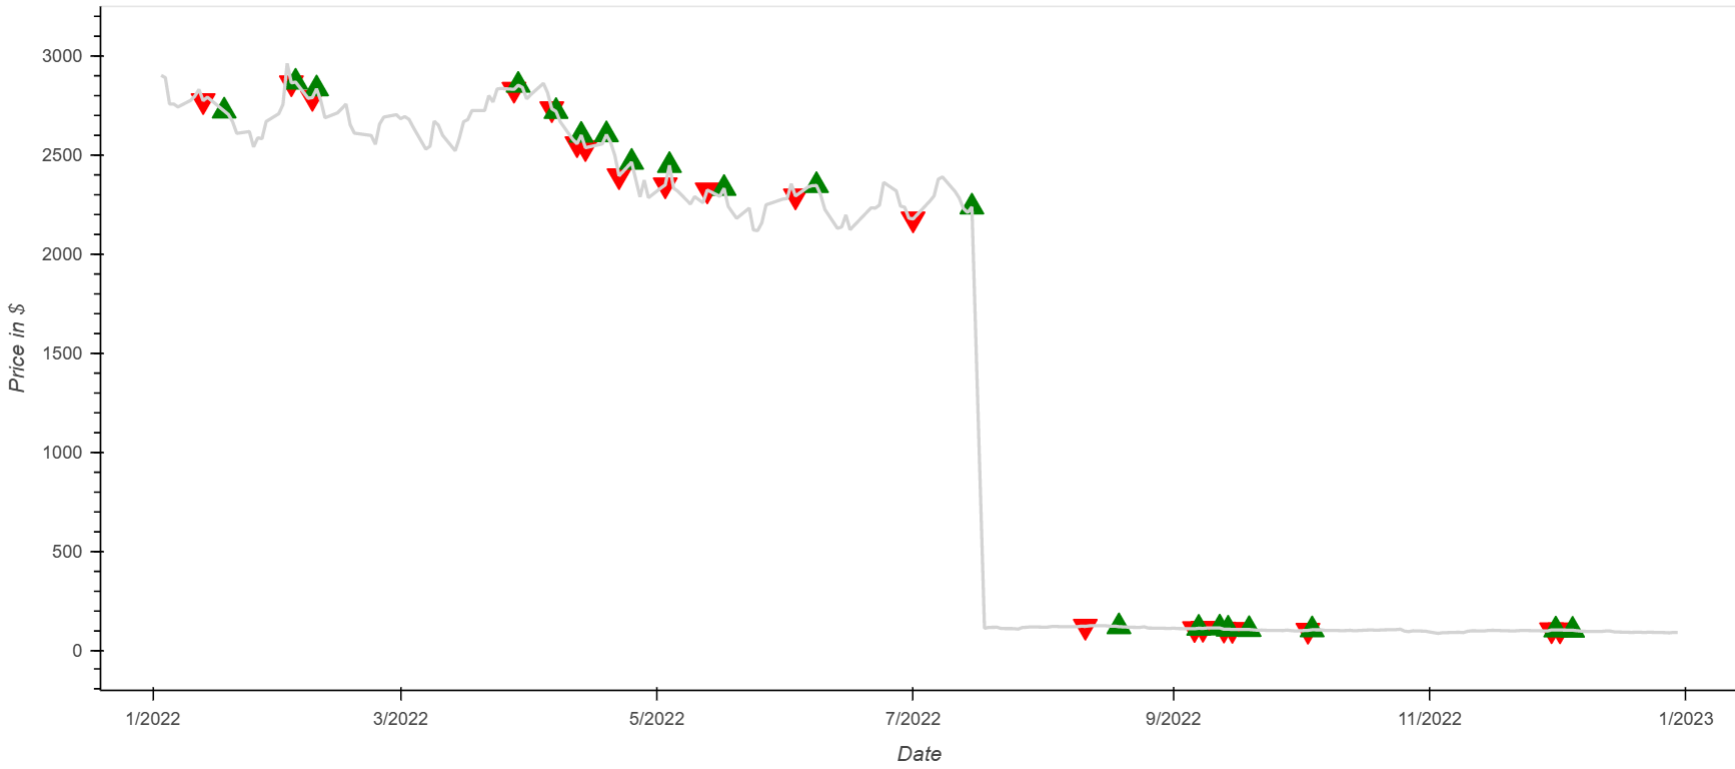
\includegraphics[width=0.8\textwidth]{Images/google_williams_R_1.png}
\caption{Entry and Exit Points for GOOGL (Lookback Period = 14 Days, Breakout Percent = 20, Williams \% R Strategy, Year = 2022)}
\label{fig:entryexit1}
\end{figure}

\begin{figure}[h!]
\centering
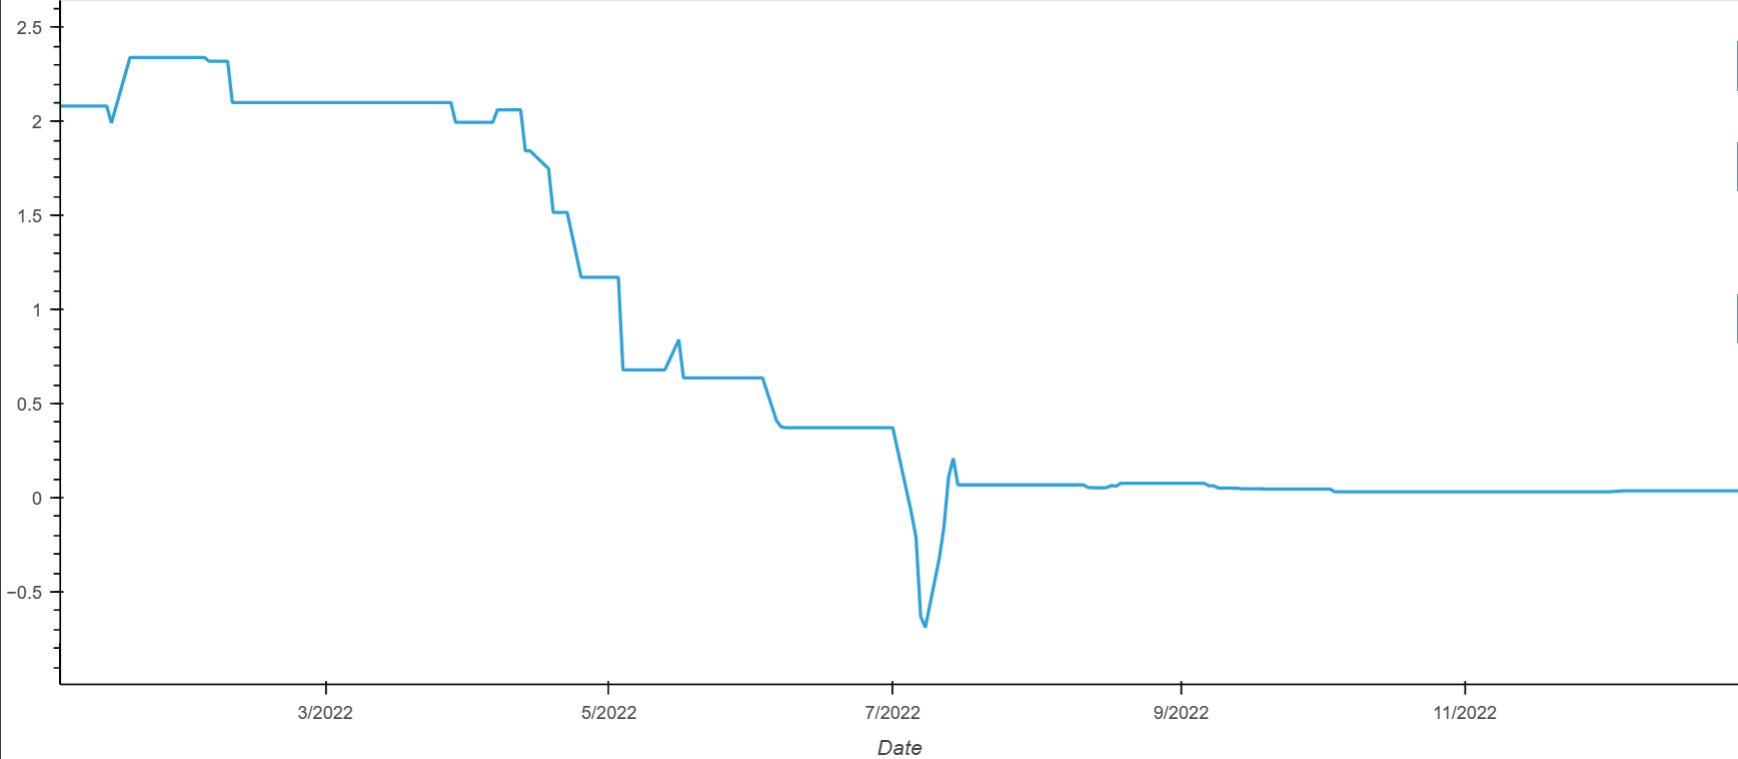
\includegraphics[width=0.8\textwidth]{Images/google_williams_R_2.png}
\caption{Cumulative Returns for GOOGL (Lookback Period = 14 Days, Breakout Percent = 20, Williams \% R Strategy, Year = 2022)}
\label{fig:entryexit1}
\end{figure}

\begin{figure}[h!]
\centering
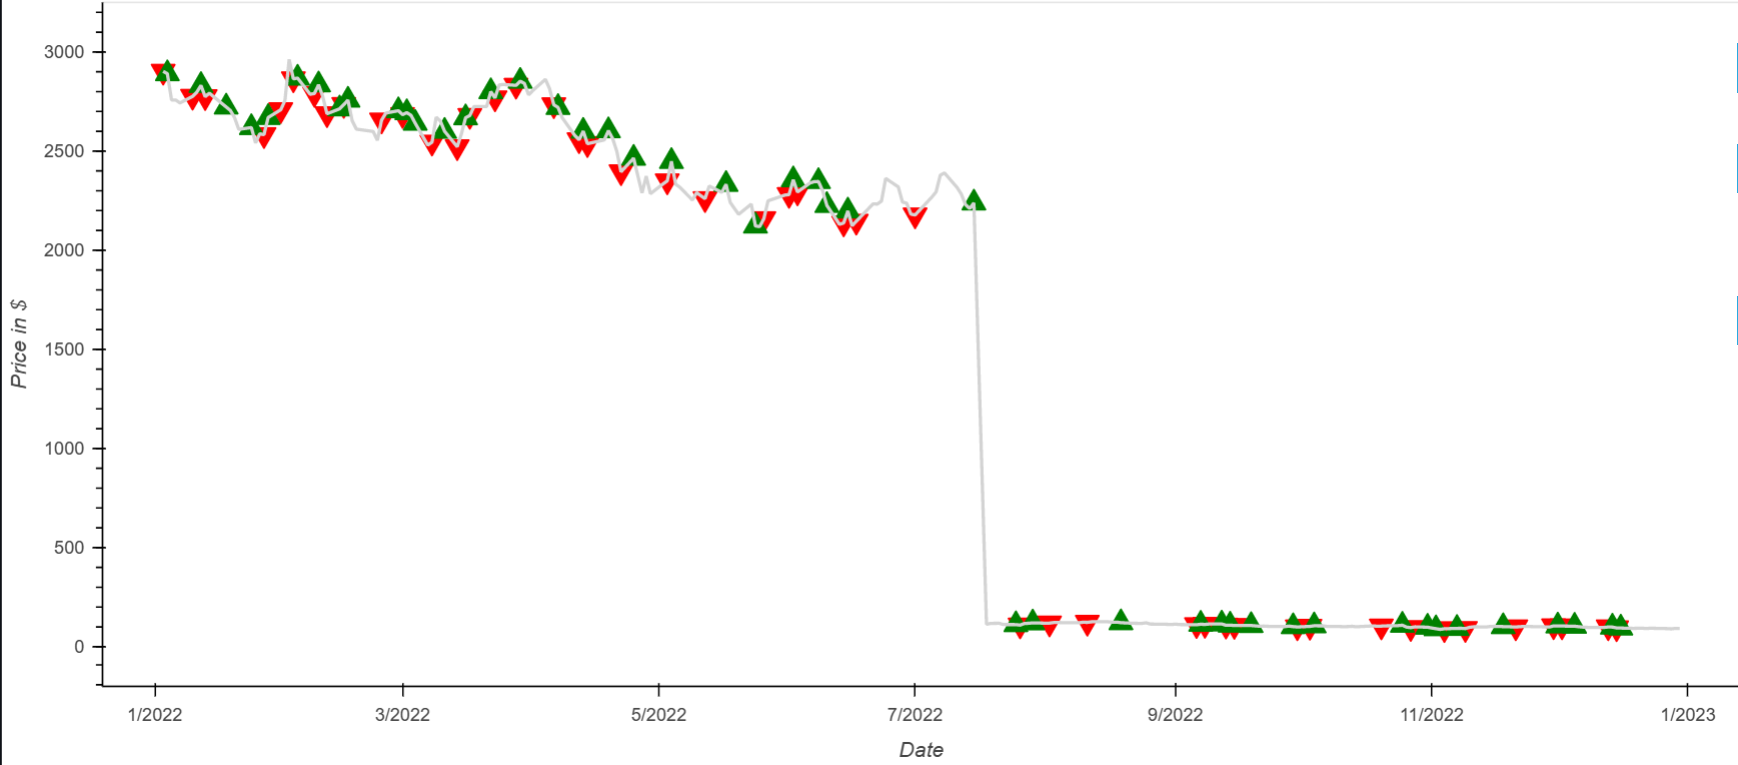
\includegraphics[width=0.8\textwidth]{Images/google_williams_lma__1.png}
\caption{Entry and Exit Points for GOOGL (Lookback Period = 14 Days, Breakout Percent = 20, Williams \% R + LMASMA Strategy, Year = 2022)}
\label{fig:entryexit1}
\end{figure}

\begin{figure}[h!]
\centering
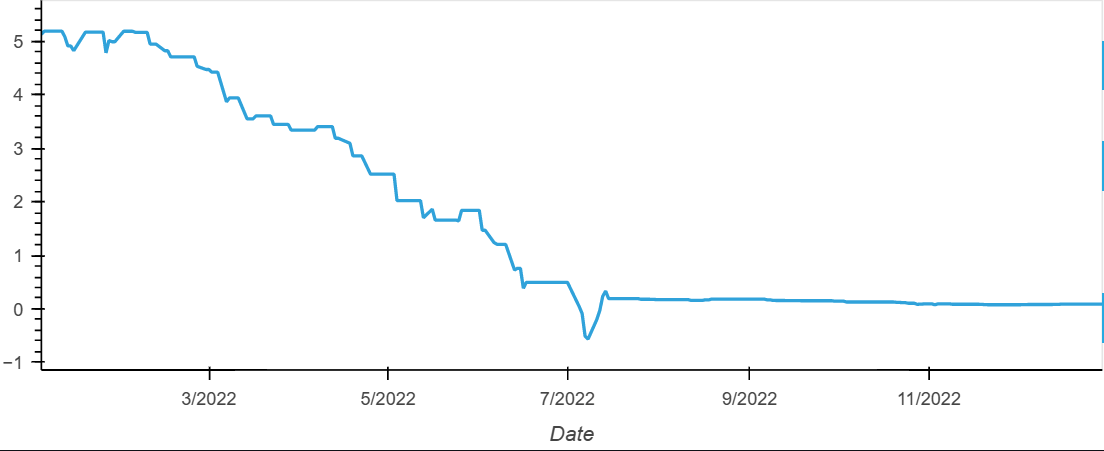
\includegraphics[width=0.8\textwidth]{Images/google_williams_lma__2.png}
\caption{Cumulative for GOOGL (Lookback Period = 14 Days, Breakout Percent = 20, Williams \% R + LMASMA Strategy, Year = 2022)}
\label{fig:entryexit1}
\end{figure}

\begin{figure}[h!]
\centering
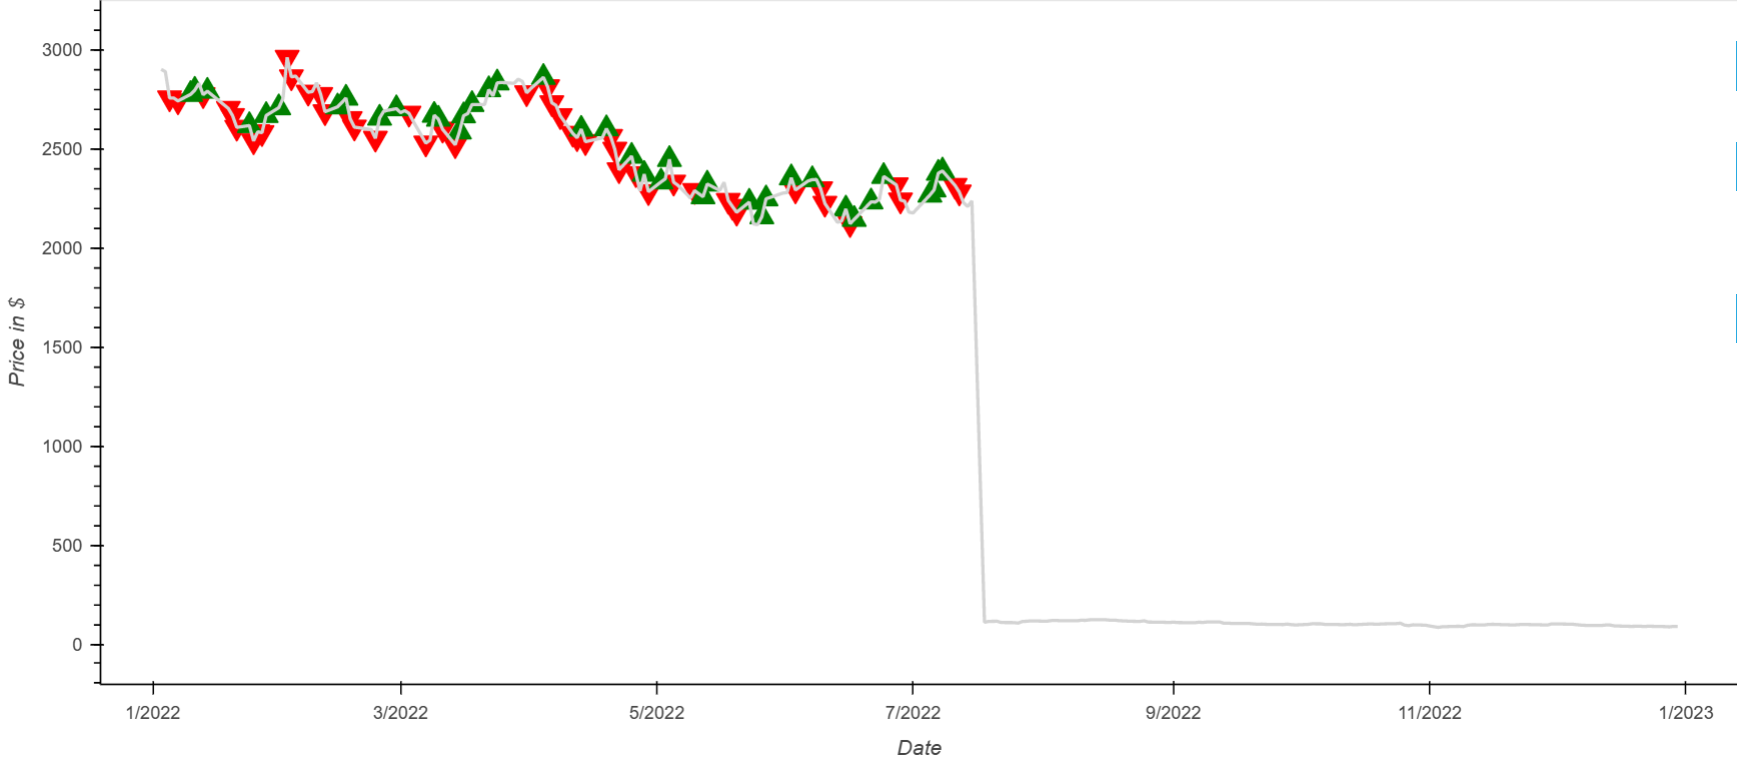
\includegraphics[width=0.8\textwidth]{Images/google_volaitity_1.png}
\caption{Entry and Exit Points for GOOGL (Lookback Period = 14 Days, Breakout Percent = 20, Volatility Breakout Strategy, Year = 2022)}
\label{fig:entryexit1}
\end{figure}

\begin{figure}[h!]
\centering
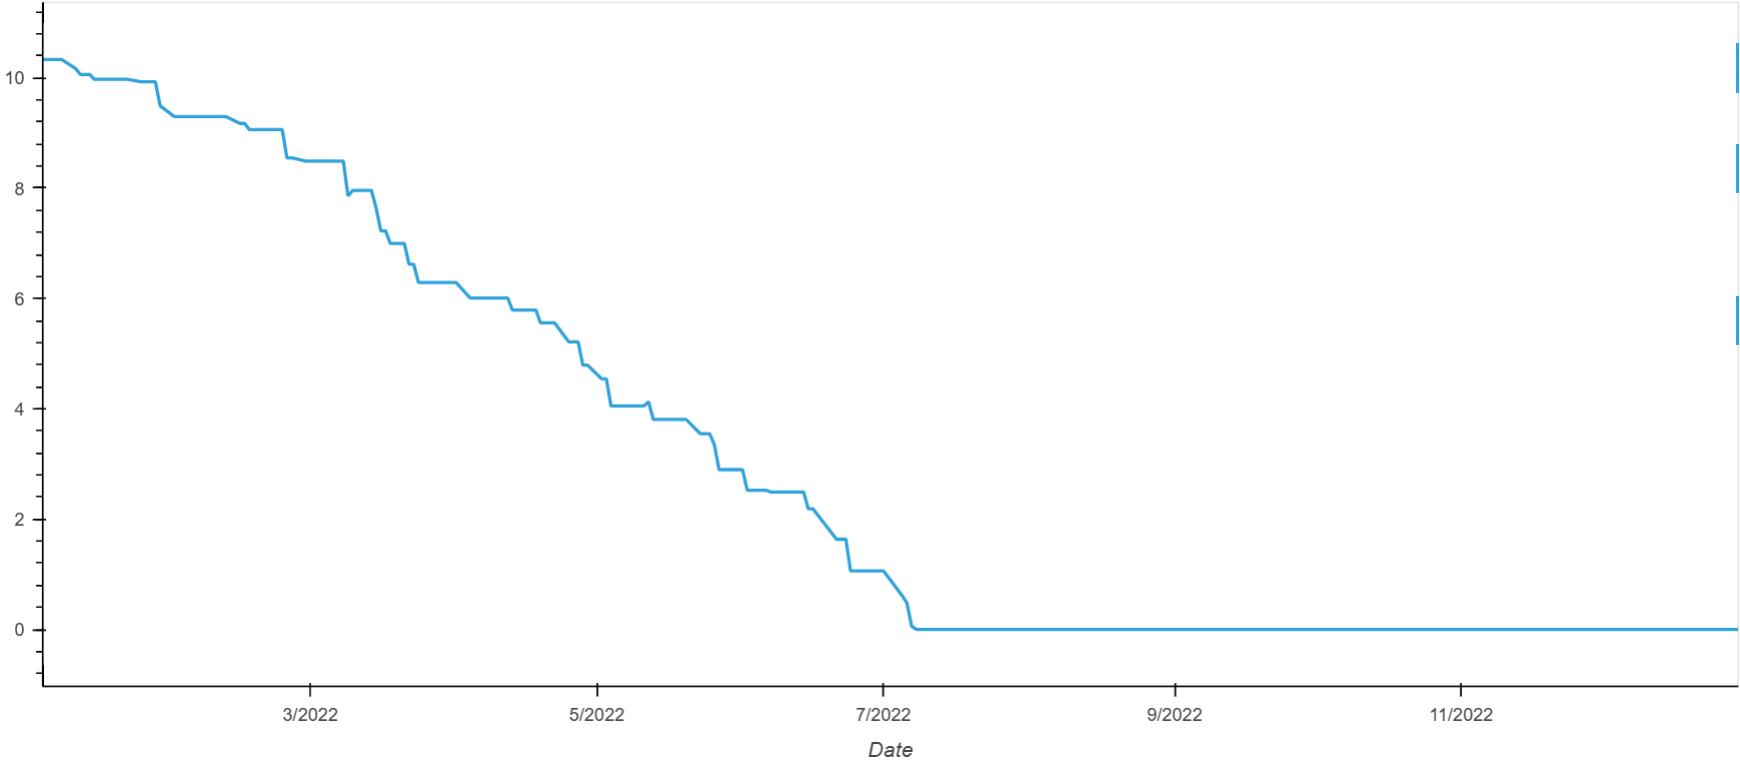
\includegraphics[width=0.8\textwidth]{Images/google_volaitity_2.png}
\caption{Cumulative Returns for GOOGL (Lookback Period = 14 Days, Breakout Percent = 20, Volatility Breakout Strategy, Year = 2022)}
\label{fig:entryexit1}
\end{figure}

\section{Backtesting Results for AAPL}
Figures show the entry and exit points for Apple with a lookback period of 14 days using the different strategy. The green arrows represent the entry points, and the red arrows represent the exit points. The blue line shows the cumulative returns of the portfolio.

The backtesting results of Apple for the year 2022 using Williams\%R+SMALMA strategy showed a positive total return of 0.012\% with a breakout percentage of 20 and a lookback period of 14 days, indicating that this strategy could potentially generate profits for short-term investors in Apple's stock market.

\begin{figure}[h!]
\centering
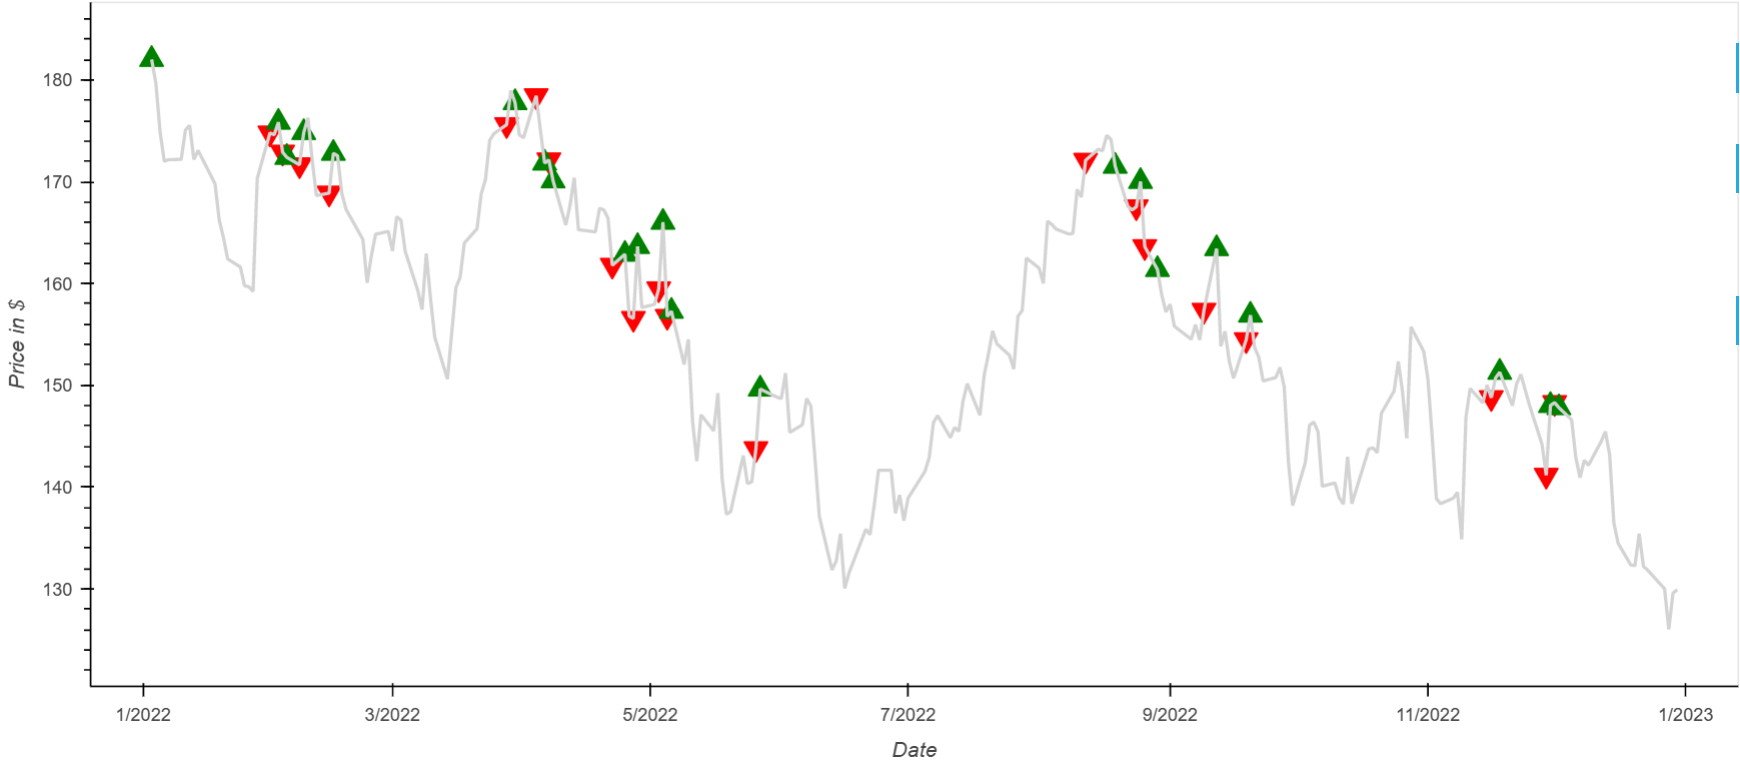
\includegraphics[width=0.8\textwidth]{Images/apple_williams_R_1.png}
\caption{Entry and Exit Points for AAPL (Lookback Period = 14 Days, Breakout Percent = 20, Williams \% R Strategy, Year = 2022)}
\label{fig:entryexit1}
\end{figure}

\begin{figure}[h!]
\centering
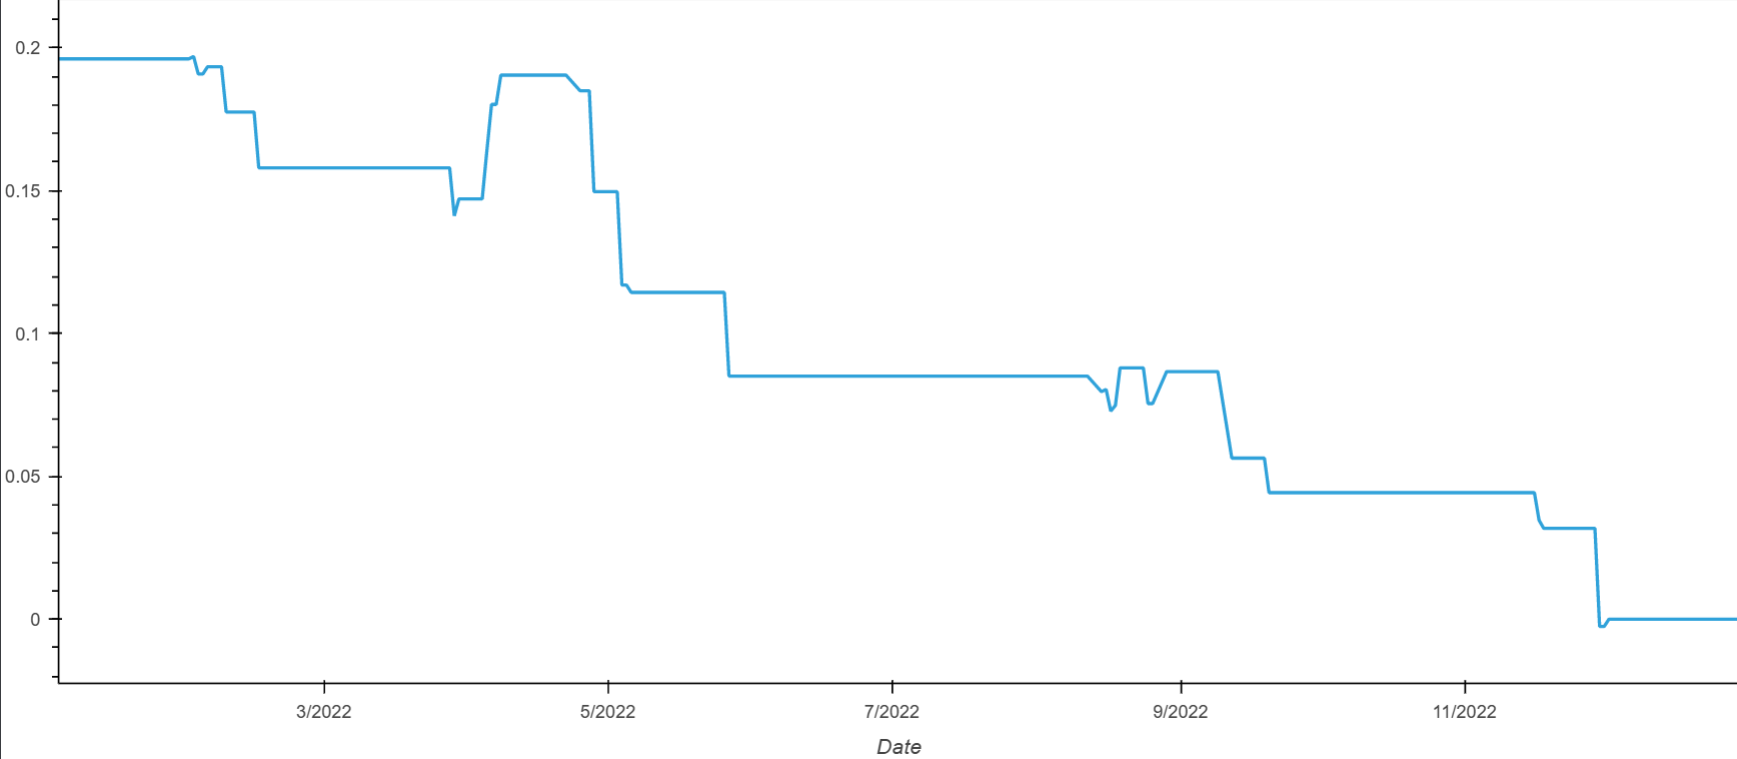
\includegraphics[width=0.8\textwidth]{Images/apple_williams_R_2.png}
\caption{Cumulative Returns for AAPL (Lookback Period = 14 Days, Breakout Percent = 20, Williams \% R Strategy, Year = 2022)}
\label{fig:entryexit1}
\end{figure}

\begin{figure}[h!]
\centering
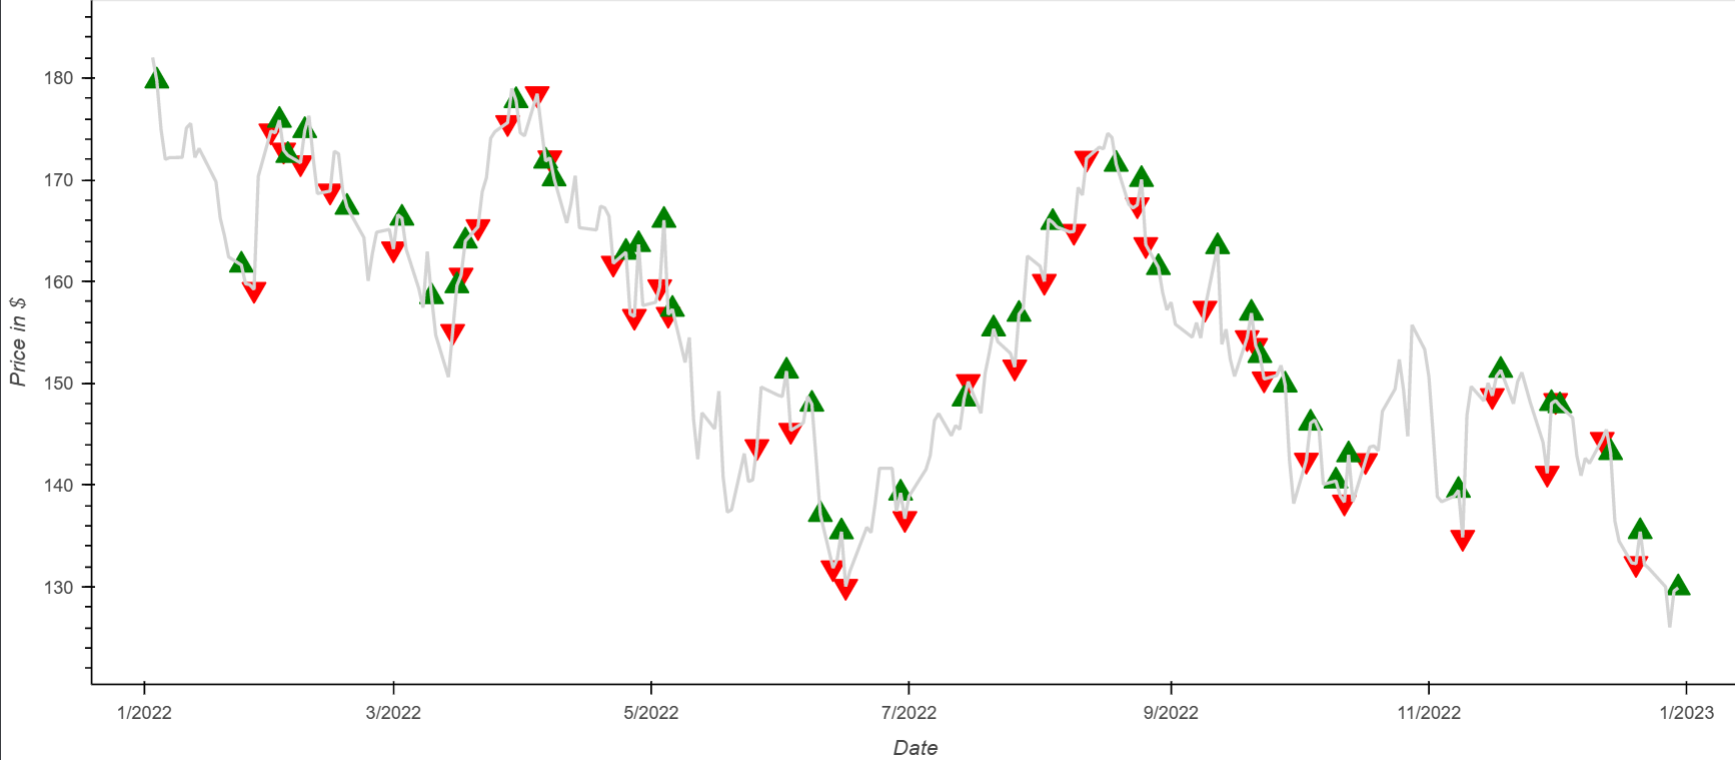
\includegraphics[width=0.8\textwidth]{Images/apple_williams_lma__1.png}
\caption{Entry and Exit Points for AAPL (Lookback Period = 14 Days, Breakout Percent = 20, Williams \% R + LMASMA Strategy, Year = 2022)}
\label{fig:entryexit1}
\end{figure}

\begin{figure}[h!]
\centering
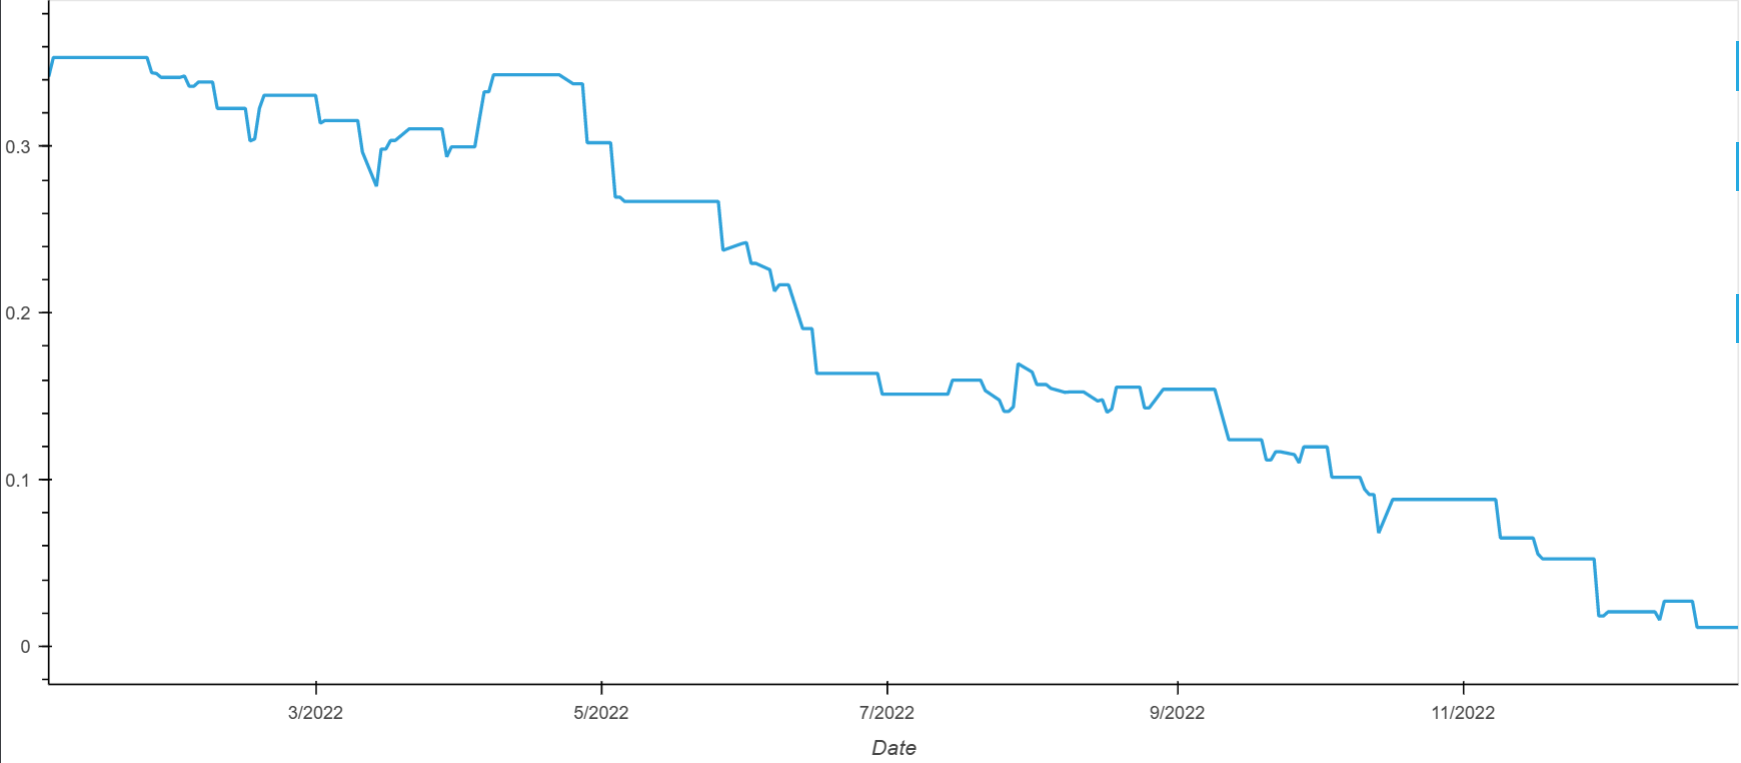
\includegraphics[width=0.8\textwidth]{Images/apple_williams_lma__2.png}
\caption{Cumulative for AAPL (Lookback Period = 14 Days, Breakout Percent = 20, Williams \% R + LMASMA Strategy, Year = 2022)}
\label{fig:entryexit1}
\end{figure} 
    % Chapter 5

\chapter{Conclusion and Future Work} % Main chapter title

\label{Chapter5} % For referencing  use \ref{Chapter5} 

\section{Conclusion}

In conclusion, the Algorithmic Trading App is a user-friendly and efficient tool that enables traders to automate their trading strategies and improve their chances of making profitable trades. By implementing different technical analysis indicators and backtesting features, the app provides users with valuable insights into market trends and helps them make informed trading decisions. Additionally, the app is designed to handle large amounts of data and execute trades in real-time, making it an ideal choice for high-frequency traders.

\section{Future Scope}

The Algorithmic Trading App has great potential for future development and enhancement. Here are a few potential areas for improvement:

\subsection{Reinforcement Learning Model}

One potential area for future development is to incorporate a reinforcement learning model for stock trading. Reinforcement Learning is a branch of machine learning that focuses on training algorithms to make decisions based on their environment. In the context of stock trading, this could be useful for creating a more adaptive trading algorithm that learns from its successes and failures. For example, the algorithm could learn to adjust its trading strategy based on market conditions, news events, or other factors that may impact stock prices. By incorporating a reinforcement learning model, the Algorithmic Trading App could potentially become more profitable and efficient.

\subsection{Sentiment Analysis Model}

Another potential area for improvement is to incorporate a sentiment analysis model to predict the impact of news and social media on the stock market. Sentiment Analysis is a process of identifying the emotional tone of a piece of text, such as a news article or social media post. By analyzing the sentiment of news articles and social media posts about a particular stock, the Algorithmic Trading App could gain valuable insights into market sentiment and make more informed trading decisions. For example, if the sentiment analysis model detects a large number of negative news articles about a particular stock, the algorithm could decide to sell that stock before its price drops further. Implementing a sentiment analysis model could help the Algorithmic Trading App stay ahead of market trends and potentially increase profits.

\subsection{Development of a Mobile App}

The Algorithmic Trading App is currently a web-based application, but developing a mobile app could provide users with greater accessibility and convenience, allowing them to trade on the go.

\subsection{Other Technical Analysis Indicators}

Technical indicators are mathematical calculations based on a stock's price and/or volume data that can be used to help identify trends, momentum, and other patterns in the stock's behavior. The Algorithmic Trading App currently incorporates a few popular technical indicators, but there are many others that could be added to enhance the algorithm's predictive power. For example, the Relative Strength Index (RSI), Moving Average Convergence Divergence (MACD), and Bollinger Bands are all widely used technical indicators that could be added to the app.

\subsection{Integration of More Data Sources}

The Algorithmic Trading App currently uses a limited number of data sources to make trading decisions. By integrating more data sources, such as social media sentiment, macroeconomic indicators, and company financial reports, the app could gain a more comprehensive view of the market and make more informed trading decisions.

\subsection{Incorporation of Risk Management Tools}

Risk management is a crucial aspect of trading, and incorporating risk management tools into the Algorithmic Trading App could help minimize losses and improve overall profitability. Examples of risk management tools include stop-loss orders, position sizing based on risk, and portfolio optimization.

\section{Limitations}

Despite its many benefits, the Algorithmic Trading App also has some limitations that should be considered. These include:

\subsection{Data Availability}

The accuracy and effectiveness of the app's trading strategies are highly dependent on the quality and availability of data. If the app is not able to access accurate and up-to-date data, it may not be able to make accurate predictions or execute trades in a timely manner.

\subsection{Market Volatility}

The stock market is a highly volatile and unpredictable environment, and even the most sophisticated trading algorithms are not immune to market fluctuations. Traders should always exercise caution and perform their own due diligence before making any trading decisions.

\subsection{Technical Issues}

Like any software application, the Algorithmic Trading App may experience technical issues or bugs from time to time. Users should be aware of these potential issues and report them to the development team as soon as possible to ensure prompt resolution. 

    % Appendix Template

\chapter*{Appendix A} 

\label{AppendixA} 

\section*{Snapshots}


\begin{figure}[ht]
    \centering
    % \begin{minipage}[b]{0.4\textwidth}
    %     \centering
    %     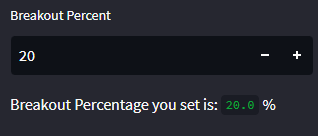
\includegraphics[width=\textwidth]{Images/breakout.png}
    %     \caption{Caption for image 1.}
    %     \label{fig:image1}
    % \end{minipage}
    % \hfill
    \begin{minipage}[b]{0.35\textwidth}
        \centering
        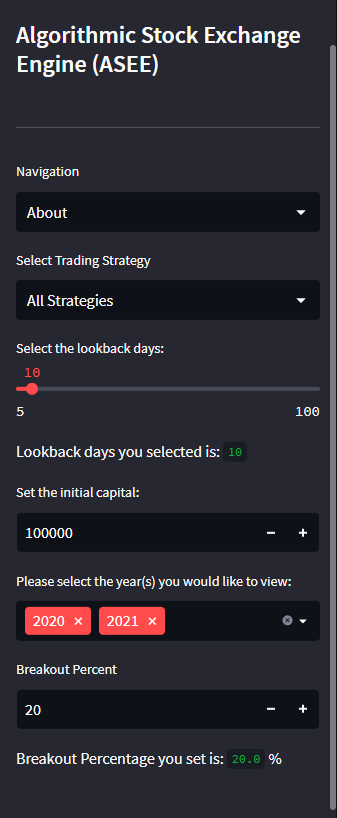
\includegraphics[width=\textwidth]{Images/sidebar.png}
        \label{fig:image2}
    \end{minipage}
    \caption{Sidebar}
    \label{fig:bothimages}
\end{figure}

\begin{figure}[ht]
    \centering
    \begin{minipage}[b]{0.4\textwidth}
        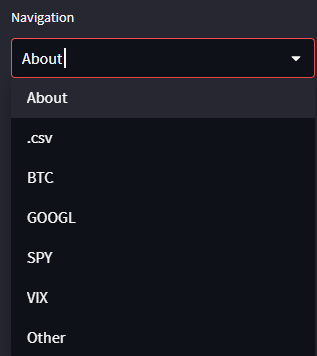
\includegraphics[width=\textwidth]{Images/navigation.png}
        \caption{Navigation Bar}
        \label{fig:image1}
    \end{minipage}
    \hfill
    \begin{minipage}[b]{0.4\textwidth}
        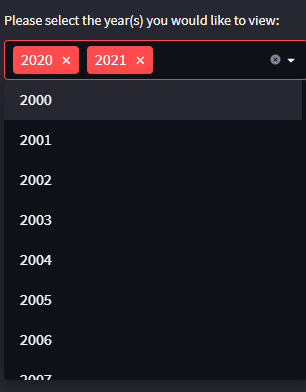
\includegraphics[width=\textwidth]{Images/year.png}
        \caption{Year Select}
        \label{fig:image1}
    \end{minipage}
    
    \begin{minipage}[b]{0.4\textwidth}
        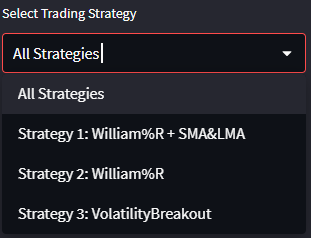
\includegraphics[width=\textwidth]{Images/strategies.png}
        \caption{Strategy Select}
        \label{fig:image2}
    \end{minipage}
    \hfill
    \begin{minipage}[b]{0.4\textwidth}
        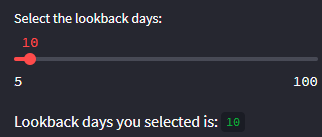
\includegraphics[width=\textwidth]{Images/lookback.png}
        \caption{Lookback Select}
        \label{fig:image2}
    \end{minipage}
    \begin{minipage}[b]{0.4\textwidth}
        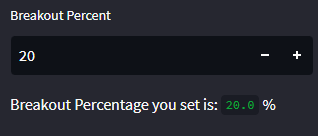
\includegraphics[width=\textwidth]{Images/breakout.png}
        \caption{Breakout}
        \label{fig:image2}
    \end{minipage}
    \hfill
    \begin{minipage}[b]{0.4\textwidth}
        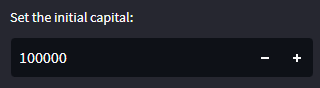
\includegraphics[width=\textwidth]{Images/capital.png}
        \caption{Capital}
        \label{fig:image2}
    \end{minipage}
    \label{fig:bothimages}
\end{figure}

    % Appendix Template

\chapter*{Appendix B} 

\label{AppendixB} 

\section*{Data Sources}

The project relied on the following data sources:

\begin{itemize}
\item \textbf{Alpha Vantage API}: This API was used to retrieve historical and real-time stock prices.
\item \textbf{News API}: This API was used to retrieve financial news related to the stocks being traded.
\end{itemize}

\section*{List of Acronyms}

\begin{itemize}
\item \textbf{API}: Application Programming Interface
\item \textbf{CSV}: Comma Separated Values
\item \textbf{SMA}: Simple Moving Average
\item \textbf{LMA}: Linear Moving Average
\item \textbf{ETF}: Exchange-Traded Fund
\item \textbf{REST}: Representational State Transfer
\item \textbf{GOOGL}: Google Ticker
\item \textbf{AAPL}: Apple Ticker
\item \textbf{MSFT}: Microsoft Ticker
\item \textbf{BTC}: Bitcoin Ticker
\end{itemize}

\section*{User Manual}

The following section provides a brief user manual for the Algorithmic Trading App:

\subsection*{Installing Dependencies}

To install the dependencies for the app, please run the following command:

\begin{lstlisting}[language=Python]
pip install -r requirements.txt
\end{lstlisting}

\subsection*{Running the App}

To run the app, please run the following command:

\begin{lstlisting}[language=Python]
streamlit run app.py
\end{lstlisting}

The app will launch in your default web browser.

\subsection*{Using the App}

Once the app is running, you will be presented with a dashboard that allows you to enter a stock symbol and view real-time and historical stock prices. You can also view and interact with the buy, sell as well as the hold signals, in order to help your portfolio. You can also apply different backtesting algorithms to backtest your strategies and improve its efficacy.

\section*{Project Timeline}

The following timeline provides a breakdown of the major milestones achieved during the project:

\begin{itemize}
\item \textbf{Week 1}: Project planning and research
\item \textbf{Week 2-3}: Data collection and preprocessing
\item \textbf{Week 4-5}: GUI development and integration with data sources
\item \textbf{Week 6-7}: Trading Strategies development and integration with GUI
\item \textbf{Week 8}: Final testing and documentation
\end{itemize}

    \bibliography{Ref}
    \cite{williams2011long}
    \cite{investopediaWR}
    \cite{williamsR}
    \cite{algorithmic_trading_python}
    \cite{lo1990}
    \cite{alphavantage}
    \cite{chande1995}
    \cite{williams1966}
    \cite{john2014}
    \cite{morton2006algorithmic}
    \cite{mendelson2018machine}
    \cite{lo2010high}
    \cite{chan2013algorithmic}
    \cite{hasbrouck2013financial}


\end{document}  
